%%%%%%%%%%%%%%%%%%%%%%%%%%%%%%%%%%%%%%%%%%%%%%%%%%%%%%%%%%%%%%%%%%%%%%%%%%%%%%%%
%%%%%%%%%%%%%%%%%%%%%%%%%%%%%%%%%%%%%%%%%%%%%%%%%%%%%%%%%%%%%%%%%%%%%%%%%%%%%%%%

\section{Estágios da musicalidade na dança}
\index{Musicalidade!Estágios da musicalidade}
\label{sec:aspectosusicalidade}
Quando estamos no percorrido de ter uma dança mais musical,
passamos por vários estágios de autoconhecimento e aprendizagem; 
dependendo da relação que conscientemente tenhamos entre a música e nosso corpo.
Neste sentido, vários dançarinos, professores e escritores,
propuseram formas de modelar por camadas ou estágios, a relação que existe entre a dança e a música.
Por exemplo, um desses modelos é indicado pelo dançarino e escritor Russell J. Hall,
que no seu blog ``Tango Words'', 
indica que podemos dançar no \hyperref[ref:Pulso]{\textbf{pulso}}, 
no \hyperref[sec:pos:Ritmo]{\textbf{ritmo}} ou na música \cite{TangoWordsEstagiosMusicalidade1}.
Por outro lado o dançarino de tango ``Paul Yang'' no seu blog ``In Search of Tango'',
ressalta que além de dançar no pulso e no ritmo, 
podemos  dançar na \hyperref[sec:pos:Melodia]{\textbf{melodia}} \cite{InSearchOfTangoEstagiosMusicalidade1}.
Em geral, podem ser achadas referencias não acadêmicas, em foros e blogs da internet,
com muitos comentários e debates sobre os estágios da musicalidade;
porem, aqui decidimos resumir e ordenar todas essas ideias num modelo com os seguintes estágios da musicalidade, $\mu(n)$,
ordenados em função do nível ($n$) de nossa relação com a música; ver Figura \ref{fig:aspectos-musica-mu}.

\begin{figure}[h!]
    \centering
    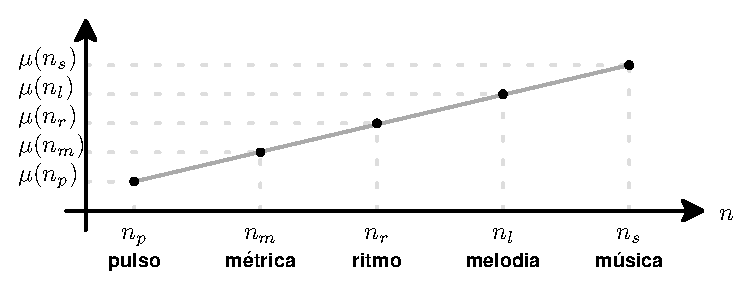
\includegraphics[width=\textwidth]{chapters/cap-musicalidade-tecnica/temporallatex-aspectos-musica-latex.eps}
    \caption{Estágios da musicalidade na dança.}
    \label{fig:aspectos-musica-mu}
\end{figure}

\begin{description}

\item[Dançar no pulso ($n_p$):] Este é um estagio inicial de nossa dança, 
que geralmente não procuramos, 
pois é onde nos encontramos, ou interiorizamos de forma inconsciente, nos primeiros dias de aula.
A maioria dos seres humanos, quando escutamos uma música, 
de forma natural podemos bater palmas ou mexer a cabeça, 
seguindo o \hyperref[ref:Pulso]{\textbf{pulso}} musical ou algum múltiplo deste. 
``Dançar no \hyperref[ref:Pulso]{\textbf{pulso}}''
implica desconhecer os acentos métricos,
e consequentemente não reconhecer os compassos, só os pulsos;
portanto, utilizar só estos como referencia na nossa dança. 
%%%
\item[Dançar na métrica ($n_m$):] 
Dançar usando a \hyperref[def:Metrica]{\textbf{métrica}}, 
implica nos movimentar com coerência com a música, 
utilizando como parâmetro de referencia a informação proporcionada pelo \hyperref[ref:Pulso]{\textbf{pulso}}, 
e os \hyperref[subsec:acentuacion1]{\textbf{tempos fortes e fracos}}; é dizer, a métrica.
Por exemplo, podemos escolher um passo com um ritmo ``rápido rápido lento'',
encaixando este dentro do compasso da música (métrica),
de modo que o movimento lento se execute no inicio do tempo forte; 
assim, se continuamos usando este movimento durante toda a música,
aconteça o que aconteça, ritmicamente ou melodicamente, na peça musical;
então estaremos só dançando na métrica.
Mais informação sobre dançar na métrica pode ser vista na Seção \ref{subsec:dancametrica}.


%%%
\item[Dançar no ritmo  ($n_r$):] Dançar usando o \hyperref[sec:pos:Ritmo]{\textbf{ritmo}},
implica movimentar-nos com coerência com a música, 
utilizando como parâmetro de seguimento 
o ritmo em alguma linha melódica ou não melódica.
Por exemplo, se percebemos  um ritmo como: \Vier \Acht \Vier  \Acht \Vier \Halb,
e nossos movimentos são realizados seguindo ele 
(ex: fazendo um movimento ao inicio de cada figura musical), então estamos dançando no ritmo.
%É importante ressaltar, que o ritmo na música tem em conta a métrica,
%pelo que se dançamos no ritmo também estamos dançando na \hyperref[def:Metrica]{\textbf{métrica}}. 
Mais informação sobre dançar no ritmo pode ser vista na Seção \ref{subsec:dancaritmo}.
 
%%%
\item[Dançar na melodia  ($n_l$):] Dançar usando a \hyperref[sec:pos:Melodia]{\textbf{melodia}},
implica algo mais que movimentar-nos seguindo variações de tempo (ritmo); 
pois na melodia se encontram as componentes \hyperref[ref:emotionsentimental]{\textbf{emocional}} 
e \hyperref[ref:emotionsentimental]{\textbf{sentimental}}, junto com a beleza, fluides e demais elementos, 
que podemos perceber numa peça musical.
É claro que todas estas percepções subjetivas, 
são gerados por aspectos da melodia como: a articulação, cadencias, ritmos, consonâncias, dissonâncias,
variações de intensidade, etc. 
Pelo que se o dançarino interpreta a informação de todos estes aspectos,
estaria sim dançando com a melodia.
%É importante ressaltar, que uma a melodia na música tem em conta o ritmo e a métrica,
%pelo que se dançamos na melodia também estamos dançando no \hyperref[sec:pos:Ritmo]{\textbf{ritmo}} e
%na \hyperref[def:Metrica]{\textbf{métrica}}.
Mais informação sobre dançar na melodia pode ser vista na Seção \ref{subsec:dancamelodia}.
%%%
\item[Dançar na música  ($n_s$):] 
Dançar usando a música implica movimentar-nos com coerência, 
seguindo os aspectos da música como, a métrica, 
o ritmo as variações de tons, tensão, articulação, etc.
Usando o fraseio e a interação entre distintas linhas melódicas;
de modo que possamos escolher informação de qualquer linha melódica ou acompanhamento,
e usar estes elementos um a um ou em simultâneo.
%Assim, seguindo esta descrição percebemos que dançar na música, 
%implica que também se está dançando na \hyperref[sec:pos:Melodia]{\textbf{melodia}}, 
%no \hyperref[sec:pos:Ritmo]{\textbf{ritmo}} e 
%na \hyperref[def:Metrica]{\textbf{métrica}}.
Mais informação sobre dançar na música pode ser vista na Seção \ref{subsec:dancamusica}.
\end{description}


Definidos estos estágios, 
devemos ressaltar que estos descrevem um processo que acontece por camadas;
é dizer que cada novo estagio do conhecimento cobre o anterior, formando um novo todo,
como é mostrado na Figura \ref{fig:aspectos-musica}.
\begin{figure}[h!]
    \centering
    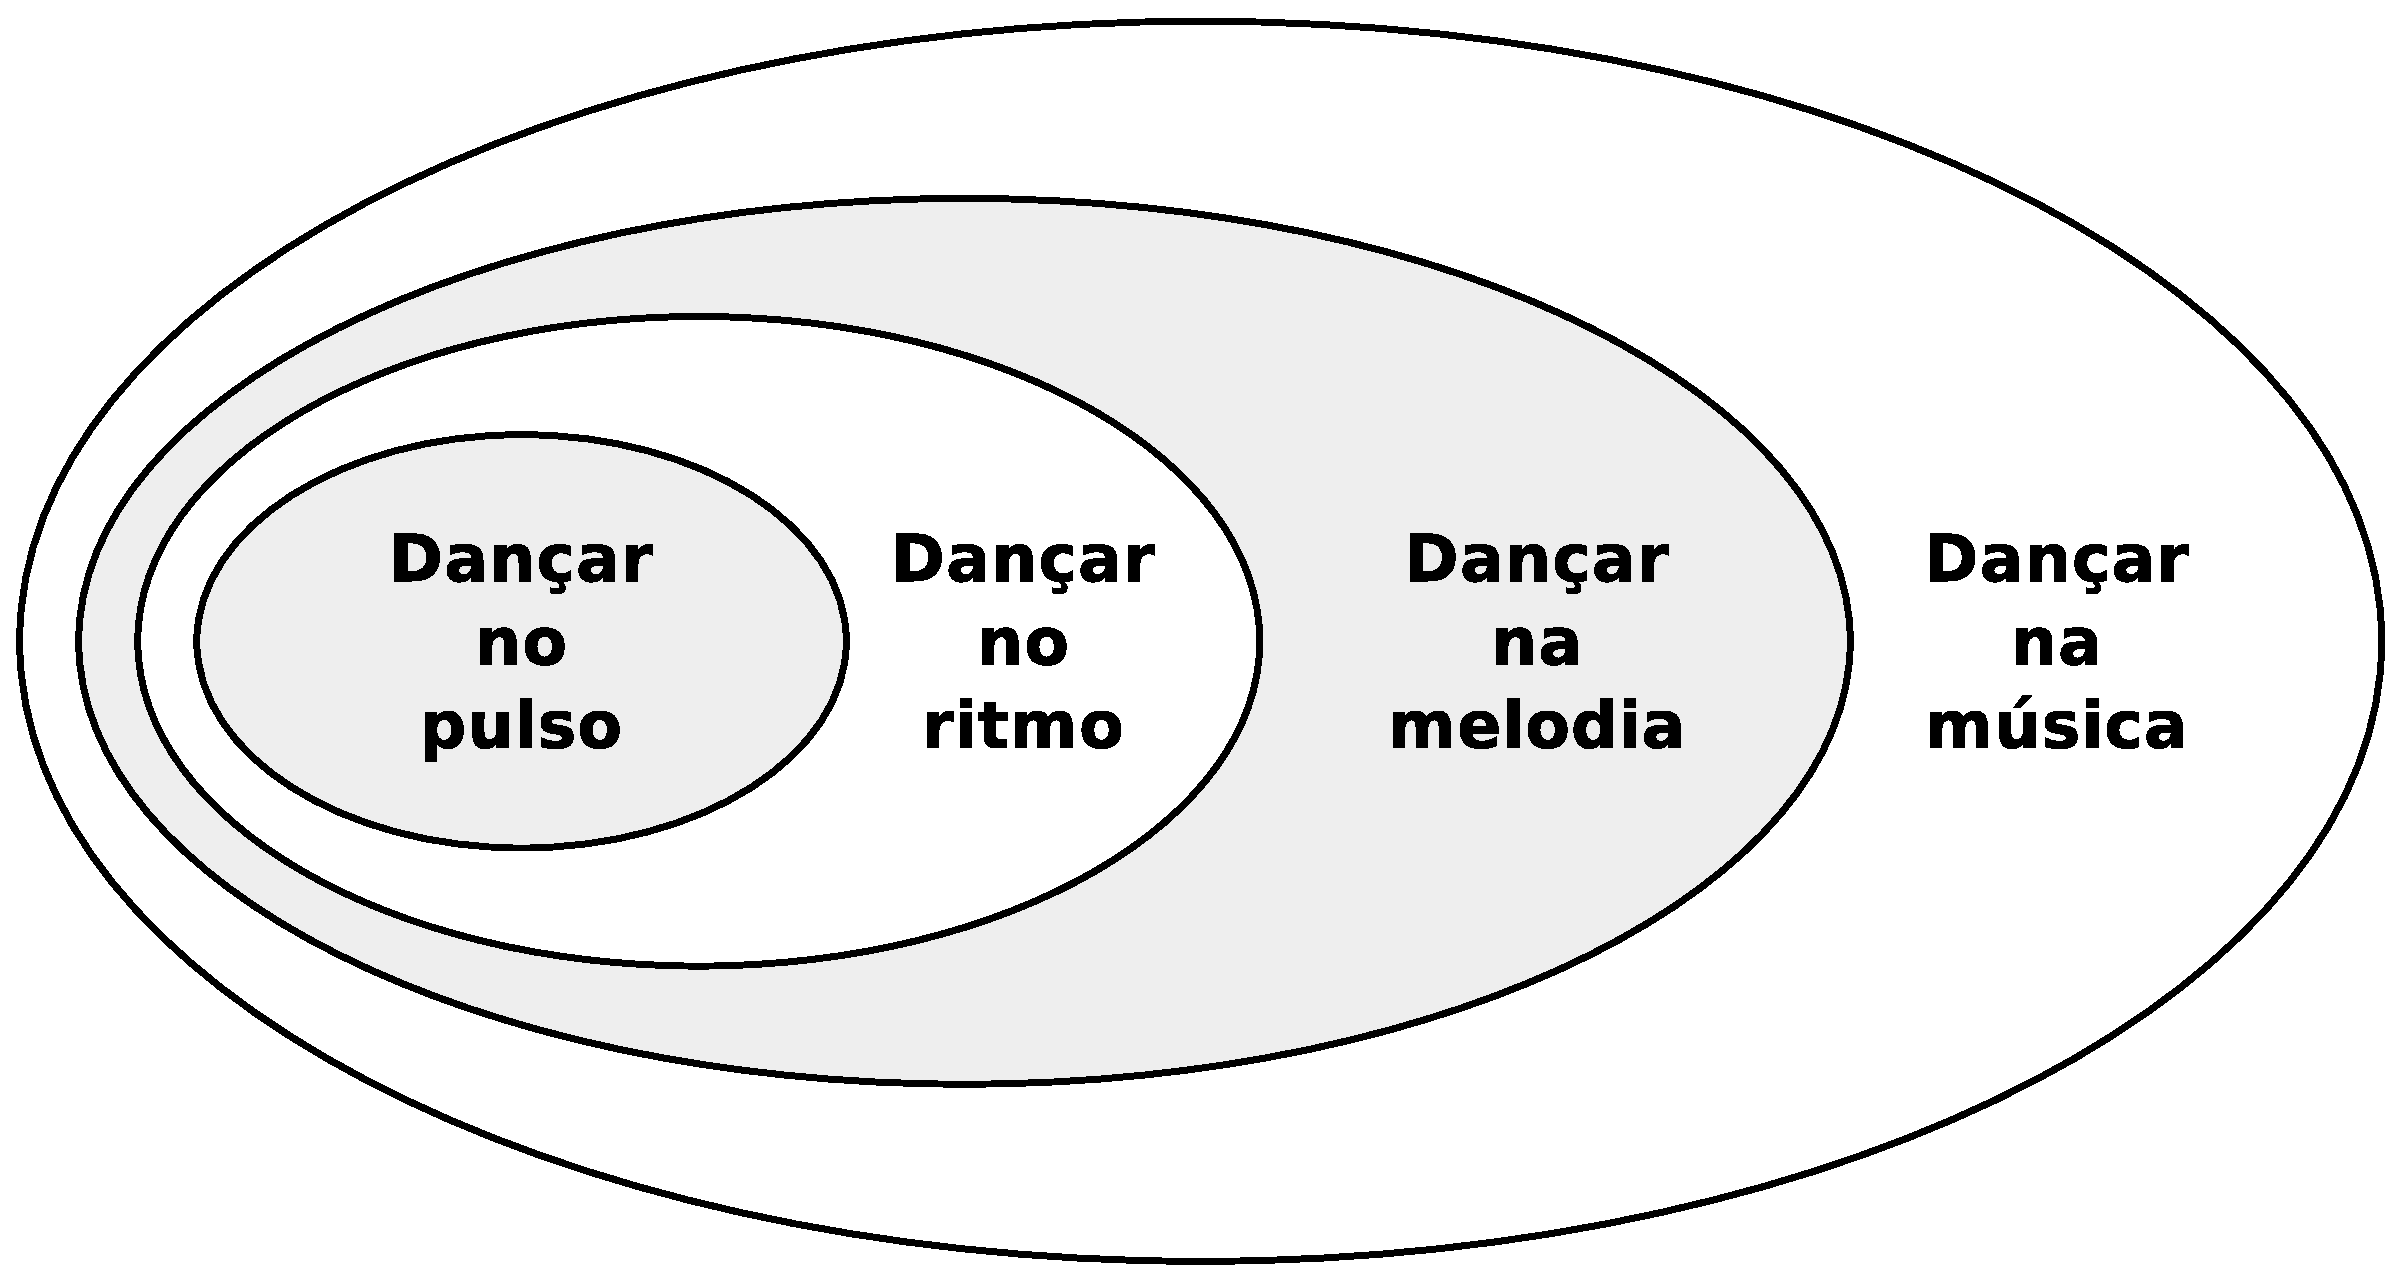
\includegraphics[width=\textwidth]{chapters/cap-musicalidade-tecnica/aspectos-musica.eps}
    \caption{Estágios da musicalidade na dança.}
    \label{fig:aspectos-musica}
\end{figure}
Assim, seguindo esta descrição percebemos que dançar na música, 
implica que também se está dançando na \hyperref[sec:pos:Melodia]{\textbf{melodia}}, 
no \hyperref[sec:pos:Ritmo]{\textbf{ritmo}}, 
na \hyperref[def:Metrica]{\textbf{métrica}} e 
no \hyperref[ref:Pulso]{\textbf{pulso}}.



Nas seguintes seções para poder exemplificar os distintos estágios da musicalidade,
usaremos a composição musical titulada ``Lamento e consolo'',
cuja pauta é mostrada na Figura \ref{fig:lamento-e-consolo}.
Esta composição está liberada baixo a 
\hyperref[ref:licensalivre]{\textbf{licença livre}}:
\hyperref[subsec:CCBYSA]{\textbf{CC BY-SA}}.

\begin{sidewaysfigure}
    \centering
    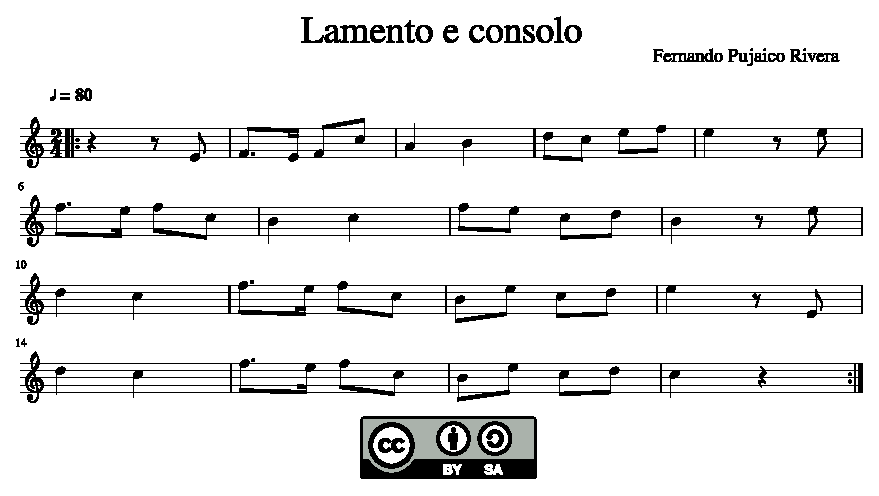
\includegraphics[width=\textwidth]{chapters/cap-musicalidade-tecnica/lamento-e-consolo-1.eps}
    \caption{Estágios da musicalidade na dança, ordenados em função de sua relação com a música.}
    \label{fig:lamento-e-consolo}
\end{sidewaysfigure}

\begin{elaboracion}[title=Pausa ativa, width= 1.0\linewidth]
\index{Musicalidade!Pausa ativa}
\label{ref:pausaativa}
Em muitos momentos de nossa dança, como quando estamos seguindo uma linha melódica,
ou algum instrumento em particular, necessitamos realizar pausas, 
já seja porque acontece um breque na música, um final de frase musical ou algum outro evento.
Para estos casos, é recomendado realizar \textbf{pausas ativas}; é dizer,
permanecer com a mente atenta à música e a nosso entorno, 
mantendo em nosso corpo um tom muscular ativo\footnote{Não 
esquecendo a postura no abraço de dança se estamos dançando a dois. }, 
para estar prontos para sair quando se reinicie a melodia.

Também, para manter a métrica da música na nossa mente,
se for necessário, 
podemos realizar leves movimentos com alguma parte de nosso corpo (cabeça, ombros, quadril, etc.),
para contar os tempos;  
de modo que poderemos souber quando iniciará o próximo tempo forte ou fraco.
Isto é importante para poder projetar o tempo de reinicio de nossa dança.
\end{elaboracion}



